\documentclass[12pt]{article}
%Mathematical TeX packages from the AMS
\usepackage{amssymb,amsmath,amsthm} 
%geometry (sets margin) 
\usepackage[margin=1.25in]{geometry}
\usepackage{enumerate}
\usepackage{graphicx}
\def\ci{\perp\!\!\!\perp}
%=============================================================
%Redefining the 'section' environment as a 'problem' with dots at the end


\makeatletter
\newenvironment{problem}{\@startsection
       {section}
       {1}
       {-.2em}
       {-3.5ex plus -1ex minus -.2ex}
       {2.3ex plus .2ex}
       {\pagebreak[3] %basic widow-orphan matching
       \large\bf\noindent{Problem }
       }
       }
       {%\vspace{1ex}\begin{center} \rule{0.3\linewidth}{.3pt}\end{center}}
       \begin{center}\large\bf \ldots\ldots\ldots\end{center}}
\makeatother


%=============================================================
%Fancy-header package to modify header/page numbering 
%
\usepackage{fancyhdr}
\pagestyle{fancy}
\lhead{Saagar Deshpande, Brandon Sim}
\chead{} 
\rhead{\thepage} 
\lfoot{\small Computer Science 182} 
\cfoot{} 
\rfoot{\footnotesize Problem Set 3} 
\renewcommand{\headrulewidth}{.3pt} 
\renewcommand{\footrulewidth}{.3pt}
\setlength\voffset{-0.25in}
\setlength\textheight{648pt}
\setlength\parindent{0pt}
%=============================================================
%Contents of problem set

\begin{document}

\title{Computer Science 182: Problem Set 3, Computational}
\author{Saagar Deshpande, Brandon Sim}

\maketitle

\begin{problem}{}
\begin{enumerate}[a.]
\item Below is a list of the symbols we are using:
\begin{enumerate}[i.]
\item C = patient is coughing
\item F = patient has a fever
\item BC = patient has blood clot
\item S = patient has stomachache
\item HBP = patient has high blood pressure
\item H = patient has headache

\item KF = patient has kidney failure
\item HF = patient has heart failure
\item BFF = patient has blood flow failure/problem
\item NF = patient has neurological system failure
\item LF = patient has liver failure
\end{enumerate}

\item Below are a set of clauses that represent this domain knowledge:

\begin{align*}
C &\rightarrow KF \lor HF\\
F &\rightarrow NF \lor BFF\\
BC &\rightarrow BFF \lor LF\\
S &\leftrightarrow KF\\
HBP &\rightarrow KF \lor BFF\\
H &\rightarrow NF \lor HF \lor KF
\end{align*}
\end{enumerate}
\end{problem}

\begin{problem}{}
\begin{enumerate}[a.]
\item Please see the file \verb|Deshpande_Sim_diagnosis.py| for our implementation of the WalkSAT algorithm.

\item 
\begin{enumerate}[i.]
\item Below are the clauses which we provide as input to our WalkSAT algorithm:

\begin{verbatim}
    Cough                   = Clause([kf, hf])
    Fever                   = Clause([nf, bff])
    Blood_clot              = Clause([bff, lf])
    Stomachache             = Clause([nkf])
    High_blood_pressure     = Clause([kf, bff])
    Headache                = Clause([nf, hf, kf])
    clauses = [Cough, Fever, Blood_clot, Stomachache,
     High_blood_pressure, Headache]
\end{verbatim}

where we use the literals as defined as follows:

\begin{verbatim}
    kf  =   Literal('kidney_failure',       False)
    hf  =   Literal('heart_failure',        False)
    bff =   Literal('bloodflow_failure',    False)
    nf  =   Literal('neuro_failure',        False)
    lf  =   Literal('liver_failure',        False)
    nkf =   Literal('kidney_failure',       True)
\end{verbatim}
These are merely translations of the propositional logic we wrote above into a form of clauses made up of literals such that our WalkSAT algorithm can understand it. We only use the right hand side, since the left hand sides are observations of the symptoms and cannot be flipped. Therefore, we know what the right hand sides must evaluate to. The explanations for each line are as follows:
\begin{enumerate}
\item We know the patient has a cough. So, either kidney failure or heart failure must be true.

\item We know the patient has a fever. So, either the neurological system has a failure or there is a problem of blood flow.

\item We know the patient has a blood clot. So, either there is a failure in blood flow or there is liver failure.

\item We know the patient does not have a stomachache. Since stomachache happens if and only if kidneys fail, we know the kidneys must not have failed (which is why we set it to True).

\item We know the patient has high blood pressure. So, either the kidneys failed or there is a blood flow problem.

\item We know the patient has a headache. So, one or more of the following systems must have failed: neurological, heart, or kidneys.
\end{enumerate}

\item Now, we run our algorithm over the parameter set $p = \{0.2, 0.8\}, \textrm{max\_flips} = \{5, 100, 5000\}$. For each parameter configuration, we run our algorithm five times. Below is a results table for these trials:
\begin{center}
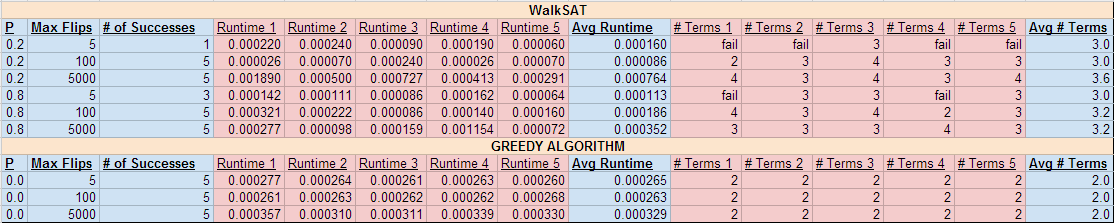
\includegraphics[width=\textwidth]{results.png}
\end{center}


\end{enumerate}
\end{enumerate}
\end{problem}

\begin{problem}{}
We changed several things about the WalkSAT algorithm to produce a version which would give the least diagnosis terms possible, while still satisfying the problem. The first is that instead of initializing all states randomly, we initialize all states to false. This makes there be more likely to be less true's in the final result, since we are flipping one state at a time and iterating, and if we start from all false's then we will likely have more false's in our final solution. In addition, we implement a fully greedy solution. Not only do we set $p = 0$ (essentially) from our original WalkSAT algorithm, we also choose greedily globally at each iterative step. That is, on each iteration, we look at each clause and see which literal should be flipped in that clause to produce the most satisfied clauses. We repeat this process over each clause, then choose to flip the literal which, compared to all other literals in all other clauses, produces the most satisfied clauses. The results, while not guaranteed to be optimal, seem much better than the original WalkSAT, as seen below:

\begin{center}
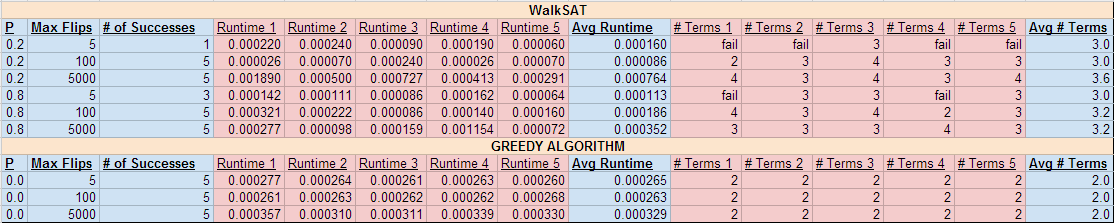
\includegraphics[width=\textwidth]{results.png}
\end{center}

Note that for our purely greedy version of the WalkSAT algorithm, we have a $100\%$ success rate for each of the 5, 100, and 5000 flips. In addition, we find the minimal diagnosis (for this problem) of two in every single case, which is clearly better than the average size of the diagnosis for the normal WalkSAT algorithm, which was over $3$ terms. However, note that although for this problem our algorithm finds the optimal (in terms of size) diagnosis, it is not guaranteed to do so on any test case because it is greedy; however, it still performs much better than the normal WalkSAT. The drawback is its runtime: because it has to check all of the clauses at each iteration, it does run much slower than its WalkSAT counterpart, as can be seen in the table. However, its ability to find the minimal diagnosis in this case consistently for all of the max flip sizes tested was impressive to us.
\end{problem}
\end{document}